\graphicspath{{content/chapters/literature_review/other_compositional_models/figures}}

\section{Other Compositional Models}
\label{sec:other_compositional_models}

This section will explore \gls{nmn} models that come after the previously explored models but are still noteworthy due to improvements they make upon the original models.
Such models may either expand upon the neural module inventory with new module types or introduce structural changes to the model architecture.
In all cases, they will demonstrate unique advancements over those models discussed previously which propose new research interests within the \gls{nmn} domain.

\subsection{NMNs\pm}
\label{subsec:nmn_plus_minus}

\citeauthor{chen_teaching_2022}\cite{chen_teaching_2022} introduced NMNs\pm as an augmented \gls{nmn} which can perform basic arithmetic operations on questions.
The model supports addition and subtraction modules --- which take up to three number arguments --- and a date comparison function.
Using these additional modules, the model was able to outperform the original \gls{nmn} on an expanded text-only question-answer dataset known as DROP.
While the model is not trained on \gls{vqa} tasks, it would be safe to assume a similar performance improvement may be expected for those \gls{vqa} tasks that require arithmetic operations (such as comparing the counts of two object types in an image).

\todo[inline]{No module overview figure, maybe include a question-answer comparison between the models? (See Figure 1 in the published paper for information.)}

\subsection{Dual-Path Neural Module Network}
\label{subsec:dual_path_neural_module_network}

\begin{figure}[htbp]
    \centering
    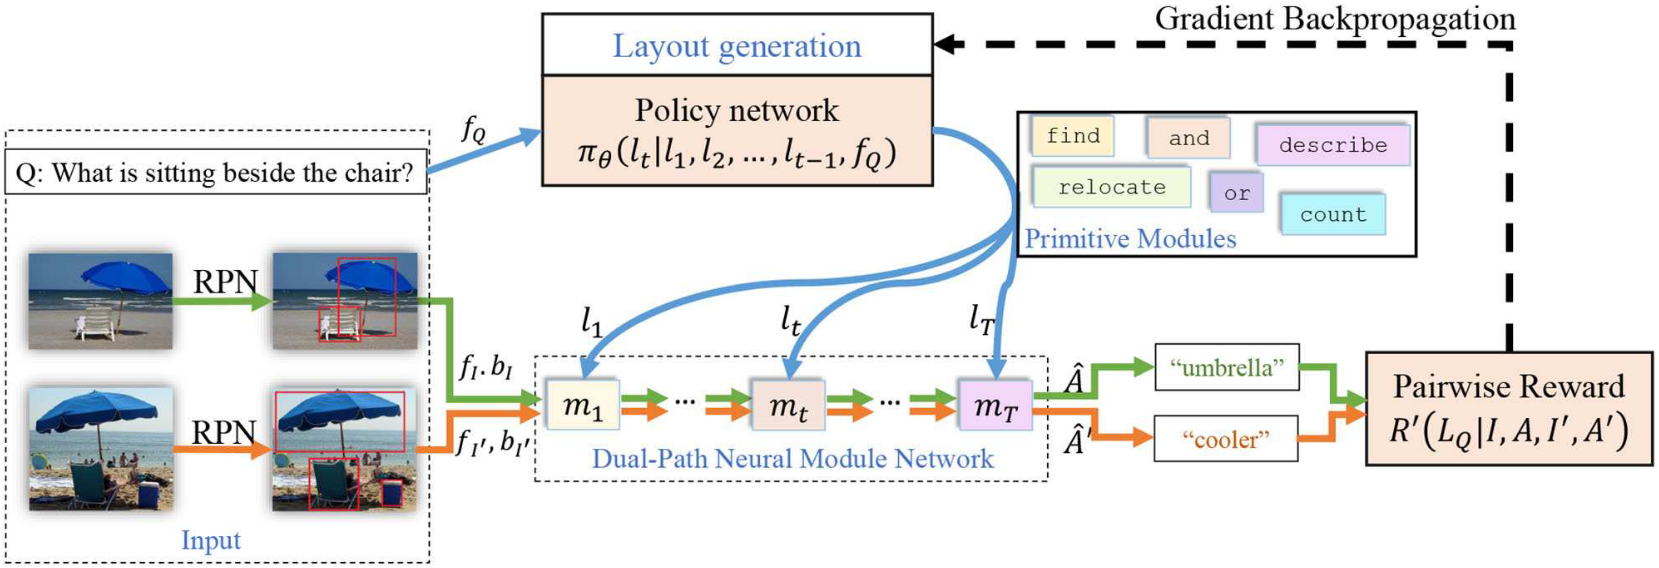
\includegraphics[width=.75\textwidth,keepaspectratio]{dpnmn_network_overview}
    \captionsource(\acrshort{dpnmn} Network Overview){Overview of the \acrshort{dpnmn} model. Each reasoning step attends to two images instead of one and processes each image in parallel, generating a pair of answers instead of a single answer. \label{fig:dpnmn_network_overview}}{\citeauthor{su_toward_2020}\cite{su_toward_2020}}
\end{figure}

The \gls{dpnmn} model was presented by \citeauthor{su_toward_2020} \cite{su_toward_2020} as an \gls{n2nmn}-based model capable of pairwise learning.
The model is capable of solving two \gls{vqa} tasks in parallel, sharing the same question but using a different image and different expected answer.
The model uses a pre-trained \glsfirst{rpn} to extract visual and spatial features from both images and feeds them into a module layout generated using a similar approach as was used by \citeauthor{hu_learning_2017} in their \gls{n2nmn}.
Instead of training using back-propagation, the model generates a reward for each pair of predicted answers and uses that to optimise the network layouts.
To reduce the likelihood of overfitting on the text semantics, a second pairwise reward is then generated if both answer predictions in a pair are correct, requiring the model to correctly discern each correct answer in the pair.

\subsection{MAC Network}
\label{subsec:mac_network}

\begin{figure}[htbp]
    \centering
    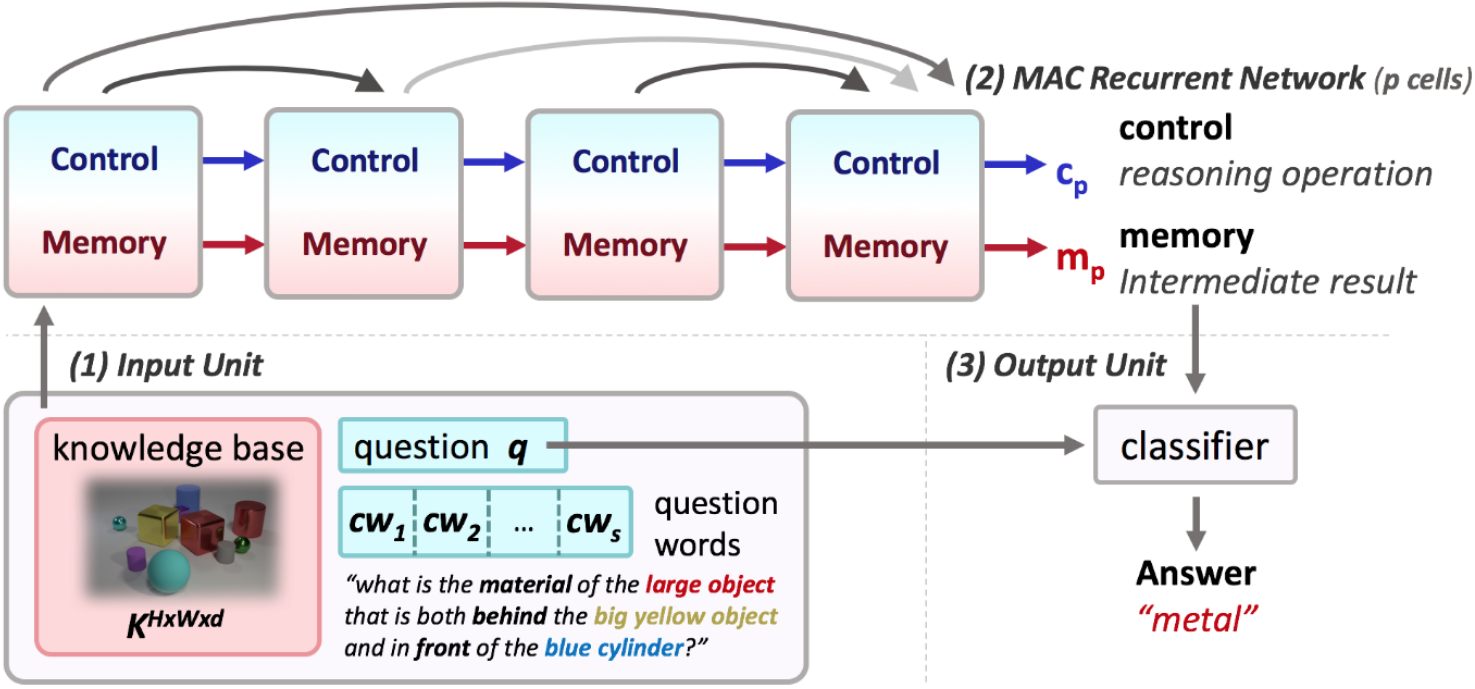
\includegraphics[width=.75\textwidth,keepaspectratio]{mac_network_overview}
    \captionsource(\acrshort{mac} Network Overview){Architecture overview of the \acrshort{mac} network model. Similar to the \gls{snmn} model, the image and question are passed to a sequence of \acrshort{mac} cells which share the intermediate results in a memory structure and a classifier uses that memory to predict the answeer. \label{fig:mac_network_overview}}{\citeauthor{hudson_compositional_2018}\cite{hudson_compositional_2018}}
\end{figure}
\begin{figure}[htbp]
    \centering
    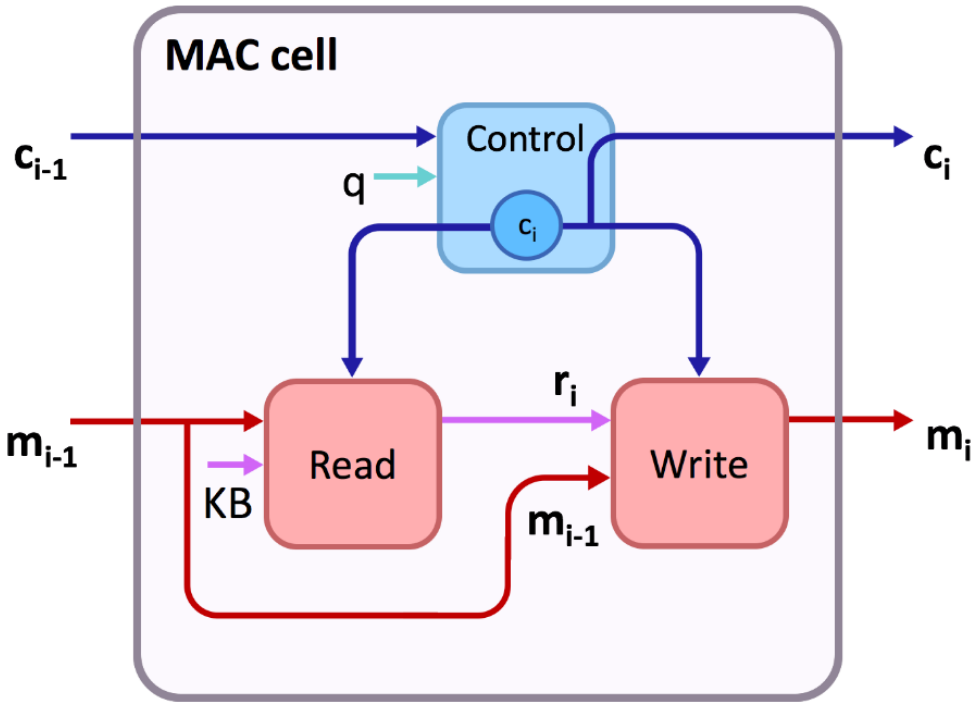
\includegraphics[width=.35\textwidth,keepaspectratio]{mac_cell_overview}
    \captionsource(\acrshort{mac} Cell Overview){Overview of a \acrshort{mac} cell, showing how it processes memory information and control state to perform reasoning and produce a new intermediate result and control state. Similar to the \gls{snmn} model, the image and question are passed to a sequence of \acrshort{mac} cells which share the intermediate results in a memory structure and a classifier uses that memory to predict the answeer. \label{fig:mac_cell_overview}}{\citeauthor{hudson_compositional_2018}\cite{hudson_compositional_2018}}
\end{figure}
\todo[inline]{Combine both figures into a single figure.}

The MAC model \cite{hudson_compositional_2018} is another such model that uses general-purpose neural cells.
It makes use of a single \gls{mac} cell at each timestep to represent each reasoning step used by the model, the structure of which can be seen in Figure~\ref{fig:mac_cell_overview}.
Each cell reads the control state and updates it according to the question and reasoning step its performing.
It then applies this controlled reasoning to the current memory state using the image features as additional input and outputs the new intermediate result to the memory state.

\subsection{Learnable Neural Module Network}
\label{subsec:learnable_neural_module_network}

\begin{figure}[htbp]
    \centering
    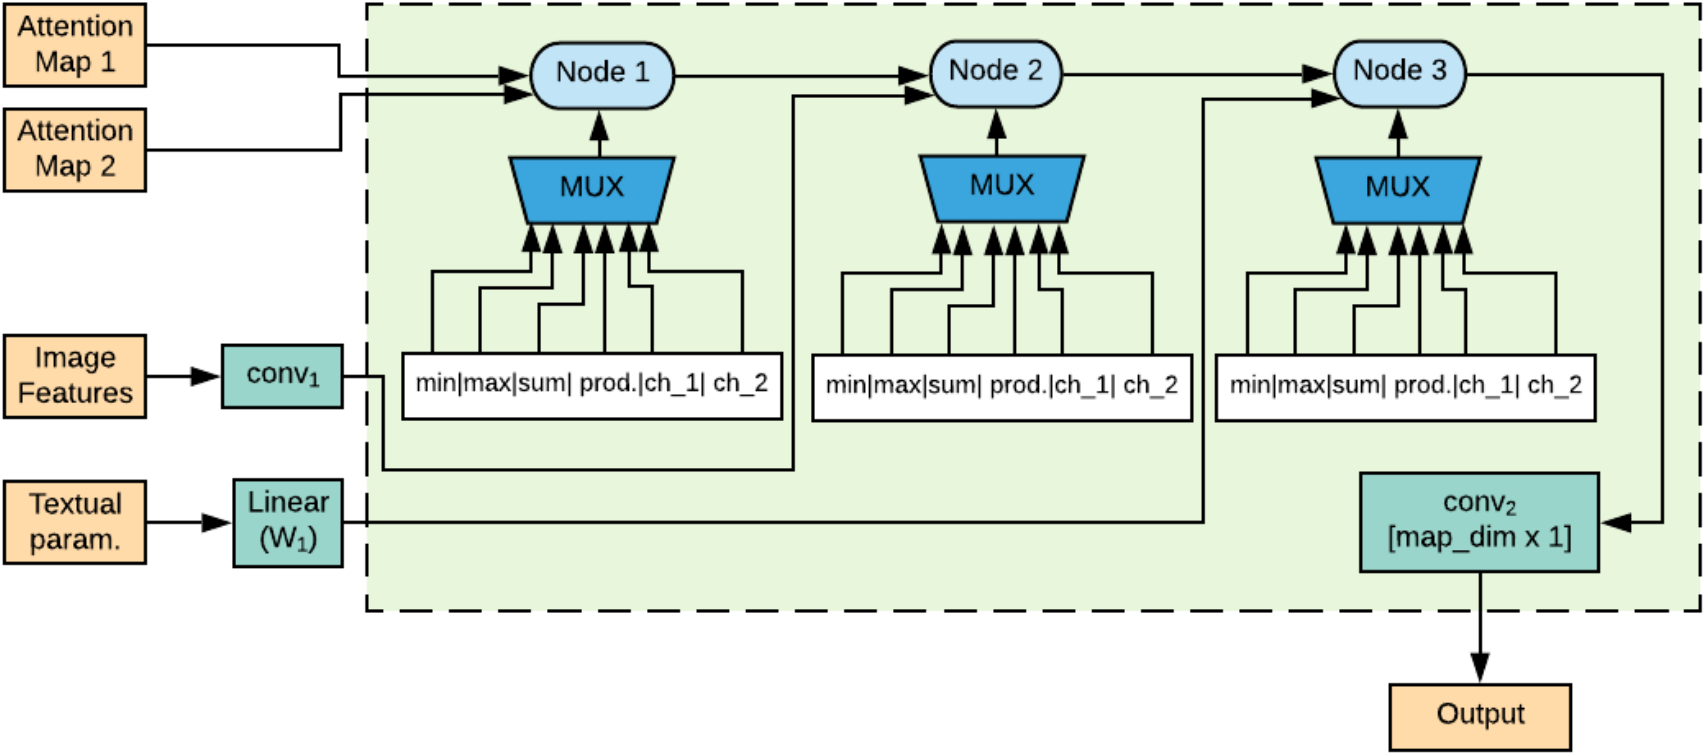
\includegraphics[width=.75\textwidth,keepaspectratio]{lnmn_module_overview}
    \captionsource(\acrshort{lnmn} Module Overview){Architecture of a 4-parameter \acrshort{lnmn} cell which accepts image features, two attention maps, and textual parameter as input \label{fig:lnmn_module_overview}}{\citeauthor{pahuja_learning_2019}\cite{pahuja_learning_2019}}
\end{figure}

Proposed by \citeauthor{pahuja_learning_2019} \cite{pahuja_learning_2019}, \gls{lnmn} is based on the \gls{snmn} model however, similar to the \gls{mmn} model, uses general-purpose neural modules instead of hard-coded ones.
The aim of this architecture was to explore the use of general-purpose neural modules as a robust and generalisable alternative to hard-coded modules and as such, does not achieve better outright performance compared to the \gls{snmn}.
Each neural module (or 'cell') is classified as either an Answer Module (outputs a memory features to be stored in the stack) or an Attention Module (outputs an attention map) and can either take 3 inputs or 4 inputs as seen in Figure~\ref{fig:lnmn_module_overview}.
Each cell contains nodes which perform internal processing of cell inputs or prior node outputs and provide
To perform training on the model weights, the model performs gradient descent on a batch from the training set.
To perform training on the model cells and architecture, the model performs an alternative gradient descent step on a random sample batch from the validation set.
This approach to training both model cells and model weights is based on \gls{darts} which is an architecture search algorithm used for training \glspl{cnn} and \glspl{rnn_g}\cite{liu_darts_2019}.
When evaluated on the CLEVR dataset, the model achieved an accuracy 1\% less than the \gls{snmn} the model was based on, despite using general-purpose modules instead of hand-tailored ones.

\todo[inline]{Paper mentions technique called Integrated Gradients for evaluating the actual performance of the cells and how well they trained. Should this be discussed?}

\subsection{Meta Module Network}
\label{subsec:meta_module_network}

\begin{figure}[htbp]
    \centering
    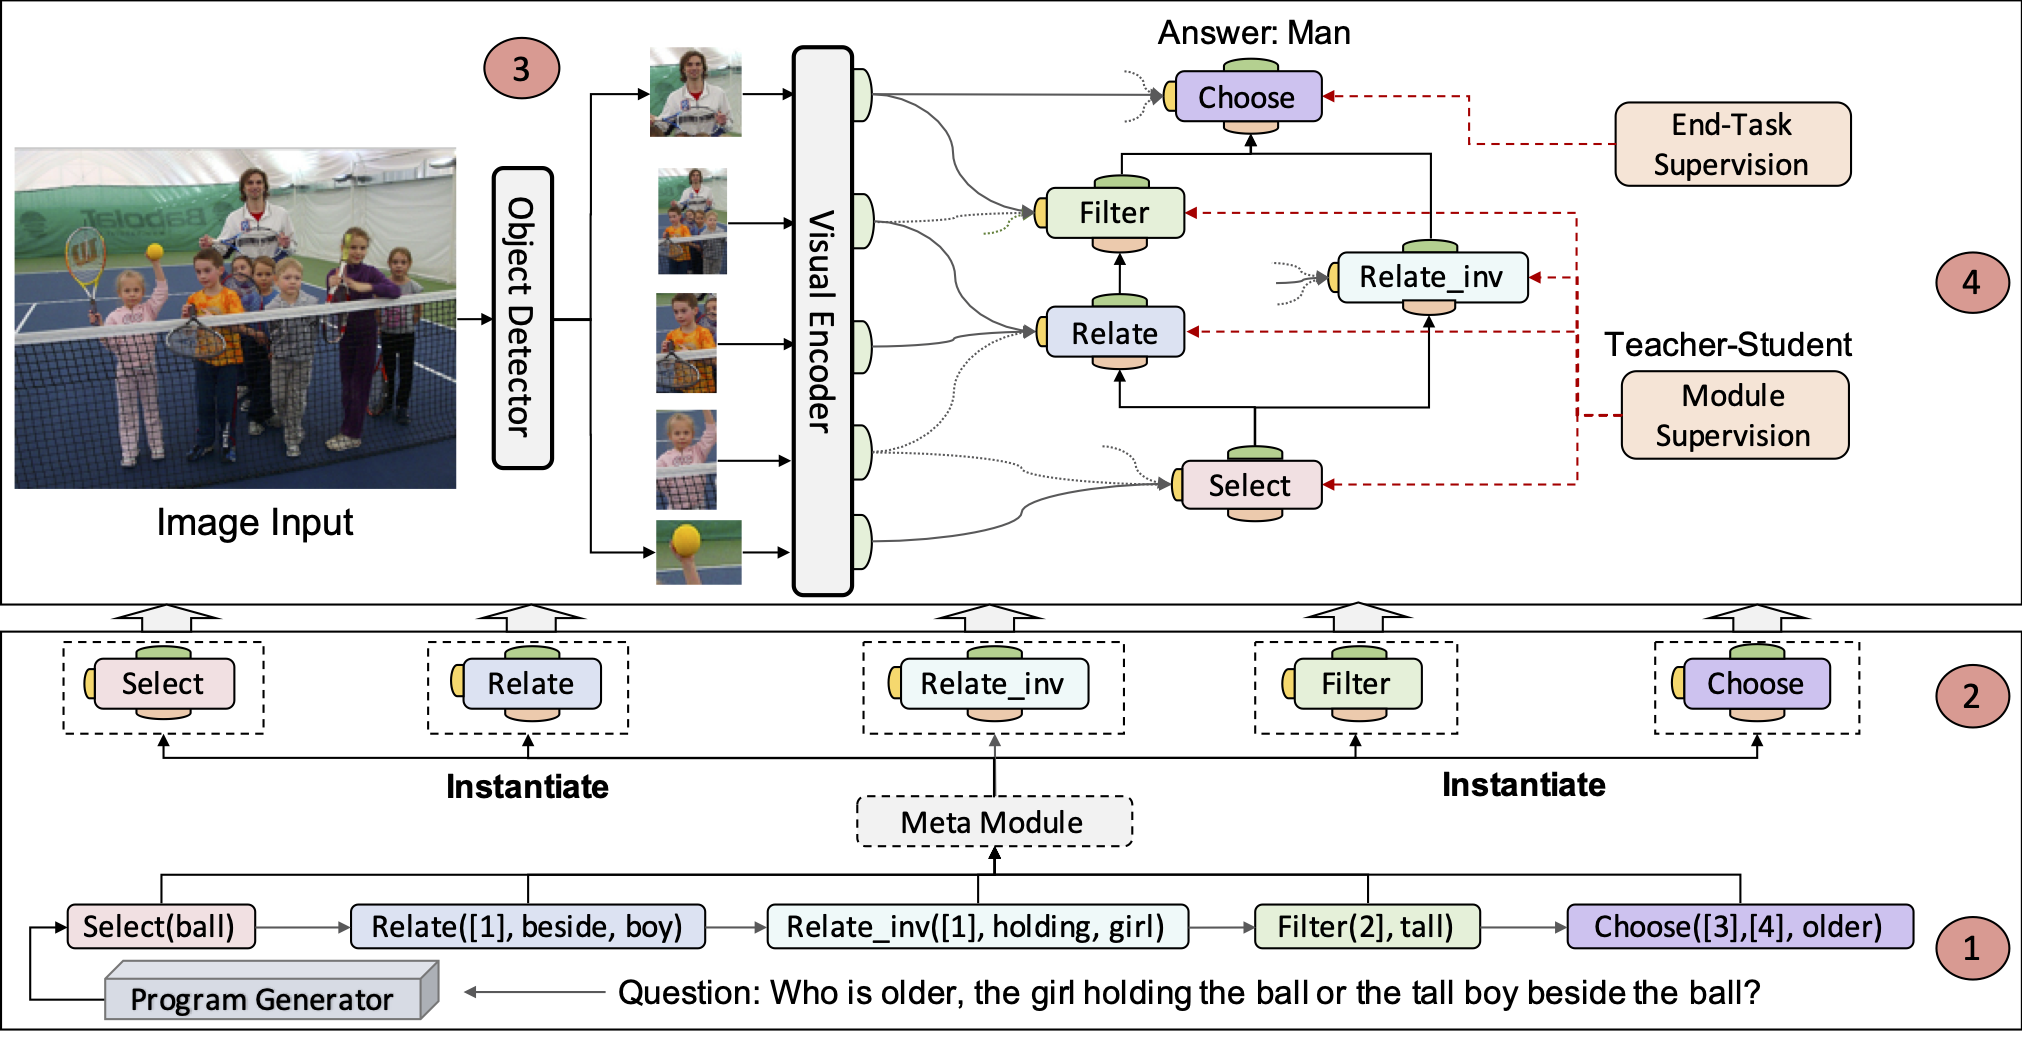
\includegraphics[width=.75\textwidth,keepaspectratio]{meta_module_network_overview}
    \captionsource(\acrshort{mmn} Overview){Architecture overview of the \acrshort{mmn} model, starting with the question-parsing (bottom) until it predicts the final answer (top) \label{fig:mmn_overview}}{\citeauthor{chen_meta_2020}\cite{chen_meta_2020}}
\end{figure}

\gls{nmn} relies on its neural modules to understand and predict answers to \gls{vqa} questions.
However, as the complexity of the questions scales up, so would the module set need to be augmented accordingly which would lead to greater complexity.
This also means the model cannot be applied to new questions which use newly-seen tasks is introduced (such as training primarily for object relationships but then being tasked with counting and object-based arithmetic).
To address this, \citeauthor{chen_meta_2020} introduced \gls{mmn} \cite{chen_meta_2020} which uses general-purpose network modules instantiated on-the-fly according to the key-value pairs provided by the model.
Given a function recipe --- denoting what task types and parameters are required for an instance of a module --- a new module is instantiated according to this spec.
Using this approach, when an unseen recipe is encountered, a new module can still be instanced using pretrained parameters and similar trained recipes.
\todo[inline]{Expand on the structure and flow of the model, maybe mention Meta Learning which partly inspired the structure of the model \ldots}


\subsection{Coreference Neural Module Network}
\label{subsec:coreference_neural_module_network}

\begin{figure}[htbp]
    \centering
    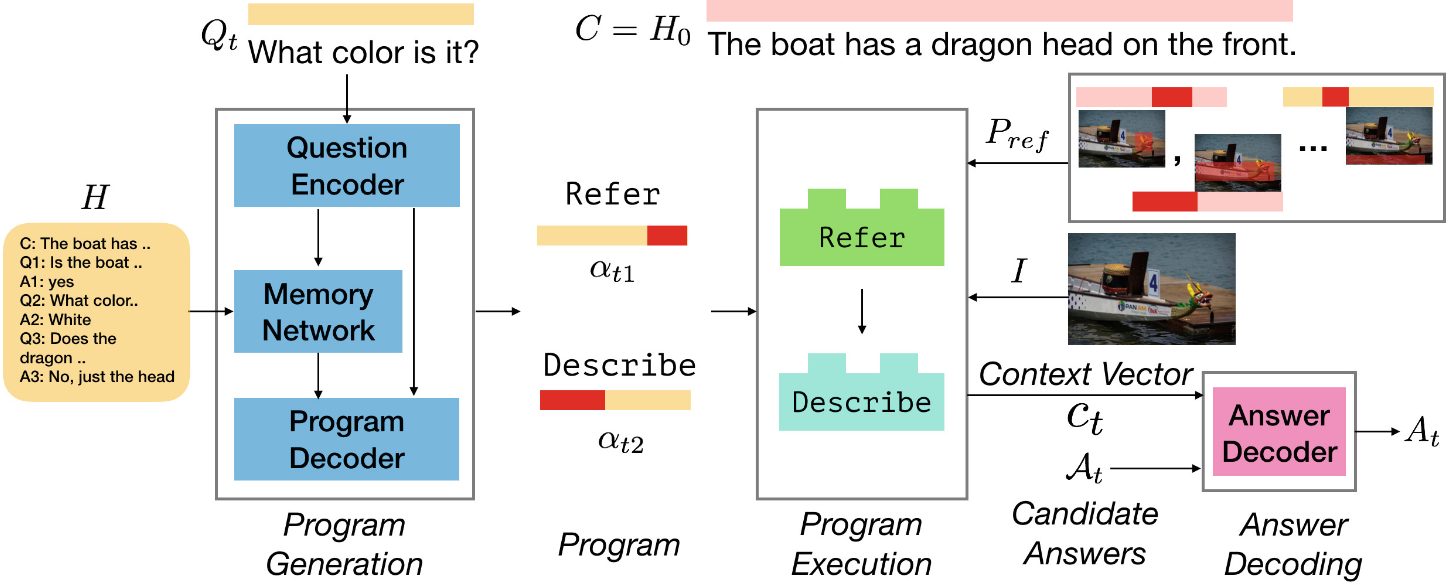
\includegraphics[width=.75\textwidth,keepaspectratio]{corefnmn_network_overview}
    \captionsource(\acrshort{corefnmn} Overview){Architecture overview of the \acrshort{corefnmn} model, with emphasis on the newly-introducde 'Refer' module and its internal function. \label{fig:corefnmn_overview}}{\citeauthor{kottur_visual_2018}\cite{kottur_visual_2018}}
\end{figure}

One of the main challenges with visual tasks discussed so far (\gls{vqa}, \gls{vcr}, and \gls{vd}) is visual coreference resolution.
Given a sentence or sentences which, when referrencing an entity, may refer to an entity more than once with more than one noun, phrase, or pronoun (eg. 'Is the lady handing her phone to her sister, the other lady' where 'lady' and 'her' both refer to one lady despite another lady being present in context).
To improve the \gls{nmn} model accuracy in detecting and handling this problem, \citeauthor{kottur_visual_2018} introduce \glsfirst{corefnmn}, an \gls{n2nmn}-based model augmented with new modules to handle \gls{vd} tasks \cite{kottur_visual_2018}.
One of the main changes to the model architecture is the introduction of a reference pool; a dictionary containing the output attention value of the 'find' modules of the program using the text parameter input as the key.
Each value in the reference pool is therefore an entity which is paired with the first word/phrase to identify it.
Using this dictionary as input, alongside a textual parameter input, a new 'Refer' module attends to the entity referred to inside the dictionary, producing a soft attention over the dictionary to select the most likely attention map.
Internally, the module measures two things; the likelihood of each key against the target text parameter, and how long its been since the target entity was last mentioned.
The softmaxed value of each key is then applied to the attention map values to obtain the final module output.
Aside from the 'Refer' module two other modules are also introduced; a 'Not' module which effectively inverts the input attention map to focus on other regions of the image, and an 'Exclude' module which looks for instances of the specified entity in the text parameter which are not found in the input attention which is also provided.
\todo[inline]{The model contains more augmentations suited to \gls{vd}. Should these be explored as well?}

\subsection{Neural Module Network for Visual Dialog}
\label{subsec:neural_module_network_for_visual_dialog}

\begin{figure}[htbp]
    \centering
    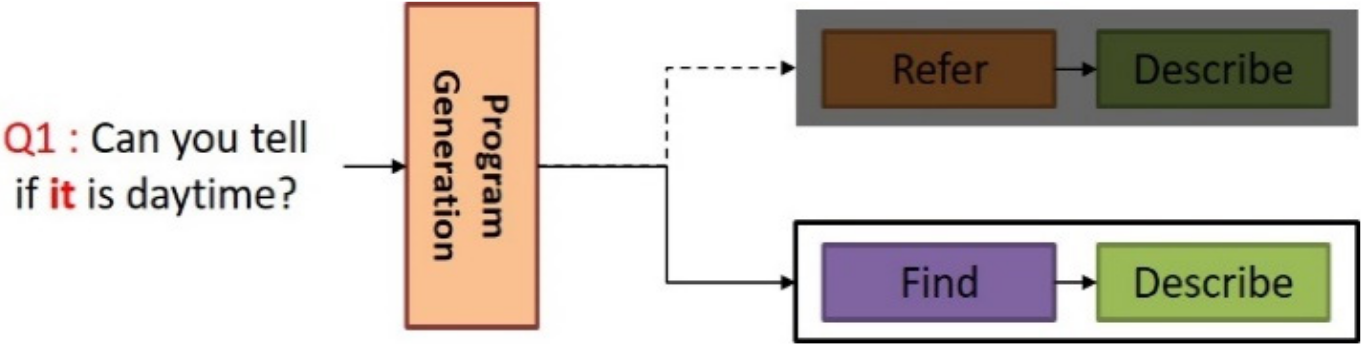
\includegraphics[width=.75\textwidth,keepaspectratio]{nmnvd_network_impersonal_pronoun}
    \captionsource(\acrshort{nmnvd} and impersonal pronouns){An overview of how the \acrshort{nmnvd} handles impersonal pronouns by avoiding the Refer module at program generation and using Find modules instead. \label{fig:nmnvd_network_impersonal_pronoun}}{\citeauthor{cho_visual_2021}\cite{cho_visual_2021}}
\end{figure}

Building upon the \gls{corefnmn} model, \citeauthor{cho_visual_2021} introduced \glsfirst{nmnvd}\cite{cho_visual_2021} which improves upon the neural module inventory and program generation of its \gls{corefnmn} predecessor.
The model builds upon the \gls{corefnmn} model by improving how the model generates programs based on impersonal pronouns.
Since impersonal pronouns refer to objects not previously encountered in dialog and would thus lead to incorrect association between the pronoun and a completely unrelated object.
To address this, the model checks for impersonal pronouns at the question stage and does not use the Refer module while still using Refer modules for personal pronouns.
Aside from this, a new output module --- known as the Compare module --- is also introduced to handle comparison tasks between two objects.
This is done by comparing the visual region containing both objects, the image features, and the textual feature parameter, to compute a final result.
Finally, the model also improves upon the Find module by using three attention iterations to produce more accurate attention regions.

\subsection{Merlot-Reserve}
\label{subsec:merlot_reserve}

\begin{figure}[htbp]
    \centering
    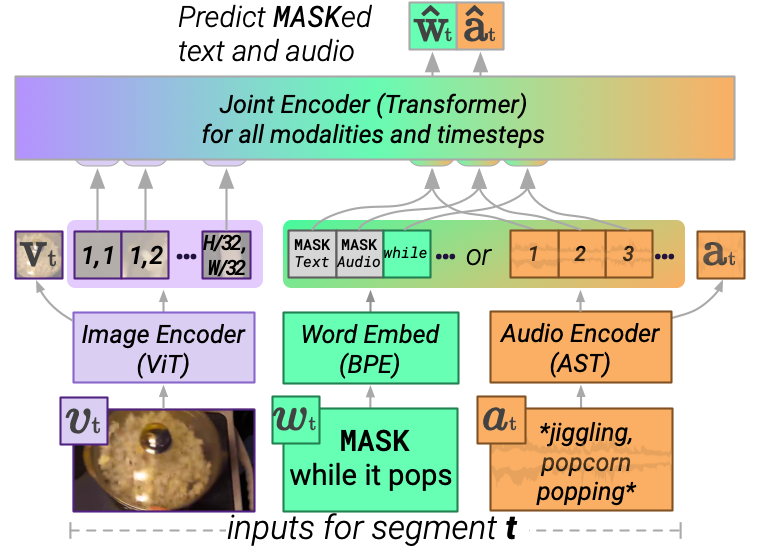
\includegraphics[width=.75\textwidth,keepaspectratio]{merlot_reserve_model}
    \captionsource(MERLOT-RESERVE model overview){An overview of the MERLOT-RESERVE model. Of particular note is it's ability to train using audio data unlike any previously-covered model. \label{fig:merlot_reserve_model_overview}}{\citeauthor{zellers_merlot_2022}\cite{zellers_merlot_2022}}
\end{figure}

To conclude, one final model which can perform \gls{vcr} tasks will be explored.
The model in question is MERLOT-RESERVE, another \gls{vcr} model by Zellers that can train on images, and either text or audio \cite{zellers_merlot_2022}.
The model is transformer-based, unlike previously-explored models which are \gls{rnn}-based, and uses a joint encoder to combine both encoded image data and word embeddings into a final prediction.
It also introduces a novel method for training called Contrastive Span Training, where the model is trained on a dataset of video-audio-subtitle entries to produce a generalised model that can be finetuned onto \gls{vcr} and other tasks\cite{zellers_merlot_2022}.
To train, each video is paired with a text/audio sequence that has a region masked out and the model must predict the correct audio or text that matches the masked as closely as possible.
The result is a model that achieved state-of-the-art results at its time\cite{zellers_merlot_2022} and still ranked among the top 15 scoring \gls{vcr} models at the time of writing this dissertation\footnote[1]{\url{https://visualcommonsense.com/leaderboard/}}.
